\documentclass[]{book}
\usepackage{lmodern}
\usepackage{amssymb,amsmath}
\usepackage{ifxetex,ifluatex}
\usepackage{fixltx2e} % provides \textsubscript
\ifnum 0\ifxetex 1\fi\ifluatex 1\fi=0 % if pdftex
  \usepackage[T1]{fontenc}
  \usepackage[utf8]{inputenc}
\else % if luatex or xelatex
  \ifxetex
    \usepackage{mathspec}
  \else
    \usepackage{fontspec}
  \fi
  \defaultfontfeatures{Ligatures=TeX,Scale=MatchLowercase}
\fi
% use upquote if available, for straight quotes in verbatim environments
\IfFileExists{upquote.sty}{\usepackage{upquote}}{}
% use microtype if available
\IfFileExists{microtype.sty}{%
\usepackage[]{microtype}
\UseMicrotypeSet[protrusion]{basicmath} % disable protrusion for tt fonts
}{}
\PassOptionsToPackage{hyphens}{url} % url is loaded by hyperref
\usepackage[unicode=true]{hyperref}
\hypersetup{
            pdftitle={Logit Models},
            pdfauthor={Bill},
            pdfborder={0 0 0},
            breaklinks=true}
\urlstyle{same}  % don't use monospace font for urls
\usepackage{natbib}
\bibliographystyle{apalike}
\usepackage{color}
\usepackage{fancyvrb}
\newcommand{\VerbBar}{|}
\newcommand{\VERB}{\Verb[commandchars=\\\{\}]}
\DefineVerbatimEnvironment{Highlighting}{Verbatim}{commandchars=\\\{\}}
% Add ',fontsize=\small' for more characters per line
\usepackage{framed}
\definecolor{shadecolor}{RGB}{248,248,248}
\newenvironment{Shaded}{\begin{snugshade}}{\end{snugshade}}
\newcommand{\KeywordTok}[1]{\textcolor[rgb]{0.13,0.29,0.53}{\textbf{#1}}}
\newcommand{\DataTypeTok}[1]{\textcolor[rgb]{0.13,0.29,0.53}{#1}}
\newcommand{\DecValTok}[1]{\textcolor[rgb]{0.00,0.00,0.81}{#1}}
\newcommand{\BaseNTok}[1]{\textcolor[rgb]{0.00,0.00,0.81}{#1}}
\newcommand{\FloatTok}[1]{\textcolor[rgb]{0.00,0.00,0.81}{#1}}
\newcommand{\ConstantTok}[1]{\textcolor[rgb]{0.00,0.00,0.00}{#1}}
\newcommand{\CharTok}[1]{\textcolor[rgb]{0.31,0.60,0.02}{#1}}
\newcommand{\SpecialCharTok}[1]{\textcolor[rgb]{0.00,0.00,0.00}{#1}}
\newcommand{\StringTok}[1]{\textcolor[rgb]{0.31,0.60,0.02}{#1}}
\newcommand{\VerbatimStringTok}[1]{\textcolor[rgb]{0.31,0.60,0.02}{#1}}
\newcommand{\SpecialStringTok}[1]{\textcolor[rgb]{0.31,0.60,0.02}{#1}}
\newcommand{\ImportTok}[1]{#1}
\newcommand{\CommentTok}[1]{\textcolor[rgb]{0.56,0.35,0.01}{\textit{#1}}}
\newcommand{\DocumentationTok}[1]{\textcolor[rgb]{0.56,0.35,0.01}{\textbf{\textit{#1}}}}
\newcommand{\AnnotationTok}[1]{\textcolor[rgb]{0.56,0.35,0.01}{\textbf{\textit{#1}}}}
\newcommand{\CommentVarTok}[1]{\textcolor[rgb]{0.56,0.35,0.01}{\textbf{\textit{#1}}}}
\newcommand{\OtherTok}[1]{\textcolor[rgb]{0.56,0.35,0.01}{#1}}
\newcommand{\FunctionTok}[1]{\textcolor[rgb]{0.00,0.00,0.00}{#1}}
\newcommand{\VariableTok}[1]{\textcolor[rgb]{0.00,0.00,0.00}{#1}}
\newcommand{\ControlFlowTok}[1]{\textcolor[rgb]{0.13,0.29,0.53}{\textbf{#1}}}
\newcommand{\OperatorTok}[1]{\textcolor[rgb]{0.81,0.36,0.00}{\textbf{#1}}}
\newcommand{\BuiltInTok}[1]{#1}
\newcommand{\ExtensionTok}[1]{#1}
\newcommand{\PreprocessorTok}[1]{\textcolor[rgb]{0.56,0.35,0.01}{\textit{#1}}}
\newcommand{\AttributeTok}[1]{\textcolor[rgb]{0.77,0.63,0.00}{#1}}
\newcommand{\RegionMarkerTok}[1]{#1}
\newcommand{\InformationTok}[1]{\textcolor[rgb]{0.56,0.35,0.01}{\textbf{\textit{#1}}}}
\newcommand{\WarningTok}[1]{\textcolor[rgb]{0.56,0.35,0.01}{\textbf{\textit{#1}}}}
\newcommand{\AlertTok}[1]{\textcolor[rgb]{0.94,0.16,0.16}{#1}}
\newcommand{\ErrorTok}[1]{\textcolor[rgb]{0.64,0.00,0.00}{\textbf{#1}}}
\newcommand{\NormalTok}[1]{#1}
\usepackage{longtable,booktabs}
% Fix footnotes in tables (requires footnote package)
\IfFileExists{footnote.sty}{\usepackage{footnote}\makesavenoteenv{long table}}{}
\usepackage{graphicx,grffile}
\makeatletter
\def\maxwidth{\ifdim\Gin@nat@width>\linewidth\linewidth\else\Gin@nat@width\fi}
\def\maxheight{\ifdim\Gin@nat@height>\textheight\textheight\else\Gin@nat@height\fi}
\makeatother
% Scale images if necessary, so that they will not overflow the page
% margins by default, and it is still possible to overwrite the defaults
% using explicit options in \includegraphics[width, height, ...]{}
\setkeys{Gin}{width=\maxwidth,height=\maxheight,keepaspectratio}
\IfFileExists{parskip.sty}{%
\usepackage{parskip}
}{% else
\setlength{\parindent}{0pt}
\setlength{\parskip}{6pt plus 2pt minus 1pt}
}
\setlength{\emergencystretch}{3em}  % prevent overfull lines
\providecommand{\tightlist}{%
  \setlength{\itemsep}{0pt}\setlength{\parskip}{0pt}}
\setcounter{secnumdepth}{5}
% Redefines (sub)paragraphs to behave more like sections
\ifx\paragraph\undefined\else
\let\oldparagraph\paragraph
\renewcommand{\paragraph}[1]{\oldparagraph{#1}\mbox{}}
\fi
\ifx\subparagraph\undefined\else
\let\oldsubparagraph\subparagraph
\renewcommand{\subparagraph}[1]{\oldsubparagraph{#1}\mbox{}}
\fi

% set default figure placement to htbp
\makeatletter
\def\fps@figure{htbp}
\makeatother

\usepackage{booktabs}
\usepackage{amsthm}
\makeatletter
\def\thm@space@setup{%
  \thm@preskip=8pt plus 2pt minus 4pt
  \thm@postskip=\thm@preskip
}
\makeatother

\title{Logit Models}
\author{Bill}
\date{2019-12-23}

\begin{document}
\maketitle

{
\setcounter{tocdepth}{1}
\tableofcontents
}
\chapter{Basics}\label{basics}

\section{Logit}\label{logit}

\[f(x)=log(\frac{p(y=1)}{1-p(y=1)})\] The basic idea of logistic
regression:
\[p(y=1)=\frac{1}{1+e^{-(\beta_0+\beta_1x_1+...+\beta_nx_n)}}=\frac{e^{\beta_0+\beta_1x_1+...+\beta_nx_n}}{1+e^{\beta_0+\beta_1x_1+...+\beta_nx_n}}\]
Thus, \(e^{\beta_0+\beta_1x_1+...+\beta_nx_n}\) can be from \(-\infty\)
to \(+\infty\), and \(p(y=1)\) will be always within the range of
\((0,1)\).

\begin{Shaded}
\begin{Highlighting}[]
\NormalTok{f<-}\ControlFlowTok{function}\NormalTok{(x)\{}\KeywordTok{exp}\NormalTok{(x)}\OperatorTok{/}\NormalTok{(}\DecValTok{1}\OperatorTok{+}\KeywordTok{exp}\NormalTok{(x))\}}
\NormalTok{data<-}\KeywordTok{seq}\NormalTok{(}\OperatorTok{-}\DecValTok{10}\NormalTok{,}\DecValTok{10}\NormalTok{,}\DecValTok{1}\NormalTok{)}
\KeywordTok{plot}\NormalTok{(data,}\KeywordTok{f}\NormalTok{(data),}\DataTypeTok{type =} \StringTok{"b"}\NormalTok{)}
\end{Highlighting}
\end{Shaded}

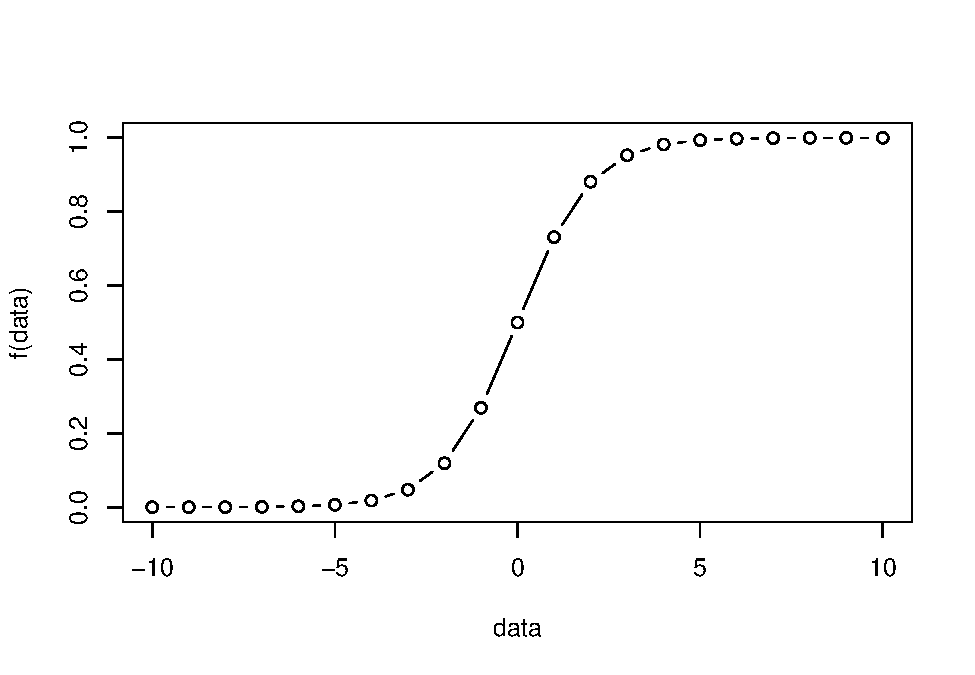
\includegraphics{bookdown-demo_files/figure-latex/unnamed-chunk-1-1.pdf}

We can also write the function into another format as follows:
\[log \frac{p(y=1)}{1-p(y=1)}= \beta_0+\beta_1x_1+...+\beta_nx_n\]

\section{Probit}\label{probit}

\[\beta_0+\beta_1x_1+...+\beta_nx_n =\Phi^{-1}(p)\] Thus,
\[\Phi(\beta_0+\beta_1x_1+...+\beta_nx_n )= p(y=1)\]

\chapter{MLE}\label{intro}

The probablity of \(y=1\) is as follows:

\[p=p(y=1)=\frac{1}{1+e^{-(\beta_0+\beta_1x_1+...+\beta_nx_n)}}=\frac{e^{\beta_0+\beta_1x_1+...+\beta_nx_n}}{1+e^{\beta_0+\beta_1x_1+...+\beta_nx_n}}\]

Thus, the likelihood function is as follows:

\[L=\prod p^{y_i}(1-p)^{1-y_i}=\prod (\frac{1}{1+e^{-(\beta_0+\beta_1x_1+...+\beta_nx_n)}})^{y_i}(\frac{1}{1+e^{\beta_0+\beta_1x_1+...+\beta_nx_n}})^{1-y_i}\]

\[=\prod (1+e^{-(\beta_0+\beta_1x_1+...+\beta_nx_n)})^{-y_i}(1+e^{\beta_0+\beta_1x_1+...+\beta_nx_n})^{-(1-y_i)}\]

Thus, the log-likelihood is as follows:
\[logL=\sum (-y_i \cdot log(1+e^{-(\beta_0+\beta_1x_1+...+\beta_nx_n)})-(1-y_i)\cdot log(1+e^{\beta_0+\beta_1x_1+...+\beta_nx_n}))\]

Typically, optimisers minimize a function, so we use negative
log-likelihood as minimising that is equivalent to maximising the
log-likelihood or the likelihood itself.

\begin{Shaded}
\begin{Highlighting}[]
\CommentTok{#Source of R code: https://www.r-bloggers.com/logistic-regression/}

\NormalTok{mle.logreg =}\StringTok{ }\ControlFlowTok{function}\NormalTok{(fmla, data)}
\NormalTok{\{}
  \CommentTok{# Define the negative log likelihood function}
\NormalTok{  logl <-}\StringTok{ }\ControlFlowTok{function}\NormalTok{(theta,x,y)\{}
\NormalTok{    y <-}\StringTok{ }\NormalTok{y}
\NormalTok{    x <-}\StringTok{ }\KeywordTok{as.matrix}\NormalTok{(x)}
\NormalTok{    beta <-}\StringTok{ }\NormalTok{theta[}\DecValTok{1}\OperatorTok{:}\KeywordTok{ncol}\NormalTok{(x)]}
    
    \CommentTok{# Use the log-likelihood of the Bernouilli distribution, where p is}
    \CommentTok{# defined as the logistic transformation of a linear combination}
    \CommentTok{# of predictors, according to logit(p)=(x%*%beta)}
\NormalTok{    loglik <-}\StringTok{ }\KeywordTok{sum}\NormalTok{(}\OperatorTok{-}\NormalTok{y}\OperatorTok{*}\KeywordTok{log}\NormalTok{(}\DecValTok{1} \OperatorTok{+}\StringTok{ }\KeywordTok{exp}\NormalTok{(}\OperatorTok{-}\NormalTok{(x}\OperatorTok\NormalTok{beta))) }\OperatorTok{-}\StringTok{ }\NormalTok{(}\DecValTok{1}\OperatorTok{-}\NormalTok{y)}\OperatorTok{*}\KeywordTok{log}\NormalTok{(}\DecValTok{1} \OperatorTok{+}\StringTok{ }\KeywordTok{exp}\NormalTok{(x}\OperatorTok\NormalTok{beta)))}
    \KeywordTok{return}\NormalTok{(}\OperatorTok{-}\NormalTok{loglik)}
\NormalTok{  \}}
  
  \CommentTok{# Prepare the data}
\NormalTok{  outcome =}\StringTok{ }\KeywordTok{rownames}\NormalTok{(}\KeywordTok{attr}\NormalTok{(}\KeywordTok{terms}\NormalTok{(fmla),}\StringTok{"factors"}\NormalTok{))[}\DecValTok{1}\NormalTok{]}
\NormalTok{  dfrTmp =}\StringTok{ }\KeywordTok{model.frame}\NormalTok{(data)}
\NormalTok{  x =}\StringTok{ }\KeywordTok{as.matrix}\NormalTok{(}\KeywordTok{model.matrix}\NormalTok{(fmla, }\DataTypeTok{data=}\NormalTok{dfrTmp))}
\NormalTok{  y =}\StringTok{ }\KeywordTok{as.numeric}\NormalTok{(}\KeywordTok{as.matrix}\NormalTok{(data[,}\KeywordTok{match}\NormalTok{(outcome,}\KeywordTok{colnames}\NormalTok{(data))]))}
  
  \CommentTok{# Define initial values for the parameters}
\NormalTok{  theta.start =}\StringTok{ }\KeywordTok{rep}\NormalTok{(}\DecValTok{0}\NormalTok{,(}\KeywordTok{dim}\NormalTok{(x)[}\DecValTok{2}\NormalTok{]))}
  \KeywordTok{names}\NormalTok{(theta.start) =}\StringTok{ }\KeywordTok{colnames}\NormalTok{(x)}
  
  \CommentTok{# Calculate the maximum likelihood}
\NormalTok{  mle =}\StringTok{ }\KeywordTok{optim}\NormalTok{(theta.start,logl,}\DataTypeTok{x=}\NormalTok{x,}\DataTypeTok{y=}\NormalTok{y, }\DataTypeTok{method =} \StringTok{'BFGS'}\NormalTok{, }\DataTypeTok{hessian=}\NormalTok{T)}
\NormalTok{  out =}\StringTok{ }\KeywordTok{list}\NormalTok{(}\DataTypeTok{beta=}\NormalTok{mle}\OperatorTok{$}\NormalTok{par,}\DataTypeTok{vcov=}\KeywordTok{solve}\NormalTok{(mle}\OperatorTok{$}\NormalTok{hessian),}\DataTypeTok{ll=}\DecValTok{2}\OperatorTok{*}\NormalTok{mle}\OperatorTok{$}\NormalTok{value)}
\NormalTok{\}}
\end{Highlighting}
\end{Shaded}

\begin{Shaded}
\begin{Highlighting}[]
\NormalTok{mydata =}\StringTok{ }\KeywordTok{read.csv}\NormalTok{(}\KeywordTok{url}\NormalTok{(}\StringTok{'https://stats.idre.ucla.edu/stat/data/binary.csv'}\NormalTok{))}
\NormalTok{mylogit1 =}\StringTok{ }\KeywordTok{glm}\NormalTok{(admit}\OperatorTok{~}\NormalTok{gre}\OperatorTok{+}\NormalTok{gpa}\OperatorTok{+}\KeywordTok{as.factor}\NormalTok{(rank), }\DataTypeTok{family=}\NormalTok{binomial, }\DataTypeTok{data=}\NormalTok{mydata)}

\NormalTok{mydata}\OperatorTok{$}\NormalTok{rank =}\StringTok{ }\KeywordTok{factor}\NormalTok{(mydata}\OperatorTok{$}\NormalTok{rank) }\CommentTok{#Treat rank as a categorical variable}
\NormalTok{fmla =}\StringTok{ }\KeywordTok{as.formula}\NormalTok{(}\StringTok{"admit~gre+gpa+rank"}\NormalTok{) }\CommentTok{#Create model formula}
\NormalTok{mylogit2 =}\StringTok{ }\KeywordTok{mle.logreg}\NormalTok{(fmla, mydata) }\CommentTok{#Estimate coefficients}


 \KeywordTok{print}\NormalTok{(}\KeywordTok{cbind}\NormalTok{(}\KeywordTok{coef}\NormalTok{(mylogit1), mylogit2}\OperatorTok{$}\NormalTok{beta))}
\end{Highlighting}
\end{Shaded}

\begin{verbatim}
##                          [,1]         [,2]
## (Intercept)      -3.989979073 -3.772676422
## gre               0.002264426  0.001375522
## gpa               0.804037549  0.898201239
## as.factor(rank)2 -0.675442928 -0.675543009
## as.factor(rank)3 -1.340203916 -1.356554831
## as.factor(rank)4 -1.551463677 -1.563396035
\end{verbatim}

\chapter{Twitter Example}\label{twitter-example}

The following is part of my course project for Stat 536. It aims to
replicate part of the findings from Barbera (2015) Birds of the Same
Feather Tweet Together: Bayesian Ideal Point Estimation Using Twitter
Data. Political Analysis 23 (1). Note that, the following model is much
simpler than that in the original paper.

\section{Model}\label{model}

Suppose that a Twitter user is presented with a choice between following
or not following another target \(j \in \{ 1, ..., m\}\). Let
\(y_{j}=1\) if the user decides to follow \(j\), and \(y_{j}=0\)
otherwise.

\[y_{j}=\begin{cases} 1 & Following \\ 0 & Not Following \end{cases}\]

\[p(y_{j}=1|\theta) = \frac{exp(- \theta_0|\theta_1 - x_j|^2)}{1+exp(- \theta_0|\theta_1 - x_j|^2)}\]
We additionally know the priors of \(\theta\).

\[\theta_i \sim N(0,10^2) (i = 0, 1)\]

The likelihood function is as follows.

\[L(Y|\theta)=\prod_{j=1}^{m} (\frac{exp(- \theta_0|\theta_1 - x_j|^2)}{1+exp(- \theta_0|\theta_1 - x_j|^2)})^{y_j}(1-\frac{exp(- \theta_0|\theta_1 - x_j|^2)}{1+exp(- \theta_0|\theta_1 - x_j|^2)})^{(1-y_j)}\]
Thus, the posterior is as follows.

\[L(Y|\theta) \cdot N(\theta_0|0,10) \cdot N(\theta_1|0,10)\]
\[\propto \prod_{j=1}^{m} (\frac{exp(- \theta_0|\theta_1 - x_j|^2)}{1+exp(- \theta_0|\theta_1 - x_j|^2)})^{y_j}(1-\frac{exp(- \theta_0|\theta_1 - x_j|^2)}{1+exp(- \theta_0|\theta_1 - x_j|^2)})^{(1-y_j)}\cdot exp(-\frac{1}{2}(\frac{\theta_0}{10})^2)\cdot exp(-\frac{1}{2}(\frac{\theta_1}{10})^2)\]

\section{Simulating Data of Senators on
Twitter}\label{simulating-data-of-senators-on-twitter}

Assume that we have 100 senators, 50 Democrats and 50 Republicans, who
we know their ideology. Assume that Democrats have negative ideology
scores to indicate that they are more liberal, whereas Republicans have
positive scores to indicate that they are more conservative. The
following is data simulation for senators.

\begin{Shaded}
\begin{Highlighting}[]
\CommentTok{# Republicans are more conservative, and they have positive numbers.}
\NormalTok{Republicans<-}\KeywordTok{c}\NormalTok{()}
\NormalTok{Republicans<-}\KeywordTok{rnorm}\NormalTok{(}\DecValTok{50}\NormalTok{,}\DecValTok{1}\NormalTok{,}\FloatTok{0.5}\NormalTok{)}
\NormalTok{No_Republicans<-}\KeywordTok{rep}\NormalTok{(}\DecValTok{1}\OperatorTok{:}\DecValTok{50}\NormalTok{,}\DecValTok{1}\NormalTok{)}
\NormalTok{Part_}\DecValTok{1}\NormalTok{<-}\KeywordTok{cbind}\NormalTok{(No_Republicans,Republicans)}

\CommentTok{# Democrats are more liberal, and they have negative numbers.}
\NormalTok{Democrats<-}\KeywordTok{c}\NormalTok{()}
\NormalTok{Democrats<-}\KeywordTok{rnorm}\NormalTok{(}\DecValTok{50}\NormalTok{,}\OperatorTok{-}\DecValTok{1}\NormalTok{,}\FloatTok{0.5}\NormalTok{)}
\NormalTok{No_Democrats<-}\KeywordTok{rep}\NormalTok{(}\DecValTok{51}\OperatorTok{:}\DecValTok{100}\NormalTok{,}\DecValTok{1}\NormalTok{)}
\NormalTok{Part_}\DecValTok{2}\NormalTok{<-}\KeywordTok{cbind}\NormalTok{(No_Democrats,Democrats)}
\NormalTok{Data_Elites<-}\KeywordTok{rbind}\NormalTok{(Part_}\DecValTok{1}\NormalTok{,Part_}\DecValTok{2}\NormalTok{)}
\NormalTok{Data_Elites<-}\KeywordTok{as.data.frame}\NormalTok{(Data_Elites)}
\KeywordTok{colnames}\NormalTok{(Data_Elites) <-}\StringTok{ }\KeywordTok{c}\NormalTok{(}\StringTok{"Elite_No"}\NormalTok{,}\StringTok{"Elite_ideology"}\NormalTok{)}

\KeywordTok{head}\NormalTok{(Data_Elites)}
\end{Highlighting}
\end{Shaded}

\begin{verbatim}
##   Elite_No Elite_ideology
## 1        1       1.337188
## 2        2       1.470603
## 3        3       0.538886
## 4        4       1.611851
## 5        5       1.490693
## 6        6       1.012758
\end{verbatim}

\section{Simulating Data of Conservative Users on Twitter and Model
Testing}\label{simulating-data-of-conservative-users-on-twitter-and-model-testing}

Assume that we observe one Twitter user, who is more conservative. To
simulate Twitter following data for this user, I assign this user to
follow more Republican senators. Thus, if the Metropolis Hastings
algorithm works as intended, we would expect to see a positive estimated
value for their ideology. Importantly, as we can see in the histogram
below, the estimated value indeed is positive, providing preliminary
evidence for the statistical model and the algorithm. In addition, for
the acceptance rate, we can see that the constant has a lower number
than ideology, since we only accept a constant when it is positive.

\begin{Shaded}
\begin{Highlighting}[]
\CommentTok{#This user approximately follows 45 Republican Senators and 10 Democrat Senators. }
\NormalTok{Data_user<-}\KeywordTok{as.data.frame}\NormalTok{(}\KeywordTok{matrix}\NormalTok{(}\KeywordTok{c}\NormalTok{(}\KeywordTok{ifelse}\NormalTok{(}\KeywordTok{runif}\NormalTok{(}\DecValTok{50}\NormalTok{)}\OperatorTok{<}\NormalTok{.}\DecValTok{1}\NormalTok{,}\DecValTok{0}\NormalTok{,}\DecValTok{1}\NormalTok{),}\KeywordTok{ifelse}\NormalTok{(}\KeywordTok{runif}\NormalTok{(}\DecValTok{50}\NormalTok{)}\OperatorTok{<}\NormalTok{.}\DecValTok{8}\NormalTok{,}\DecValTok{0}\NormalTok{,}\DecValTok{1}\NormalTok{))), }\DecValTok{100}\NormalTok{, }\DecValTok{1}\NormalTok{)}
\KeywordTok{colnames}\NormalTok{(Data_user)<-}\KeywordTok{c}\NormalTok{(}\StringTok{"R_User"}\NormalTok{)}
\NormalTok{Data_combined<-}\KeywordTok{cbind}\NormalTok{(Data_Elites,Data_user)}

\NormalTok{X_data<-Data_combined}\OperatorTok{$}\NormalTok{Elite_ideology}
\NormalTok{Y_data<-Data_combined}\OperatorTok{$}\NormalTok{R_User}

\NormalTok{fit_C<-}\KeywordTok{Bayes_logit}\NormalTok{(Y_data,X_data)}
\NormalTok{fit_C}\OperatorTok{$}\NormalTok{acceptance_rate}
\end{Highlighting}
\end{Shaded}

\begin{verbatim}
## [1] 0.1580790 0.5067534
\end{verbatim}

\begin{Shaded}
\begin{Highlighting}[]
\KeywordTok{plot}\NormalTok{(fit_C}\OperatorTok{$}\NormalTok{theta[,}\DecValTok{1}\NormalTok{],}\DataTypeTok{main=}\StringTok{"Constant (Conservative Users)"}\NormalTok{,}
     \DataTypeTok{xlab=}\StringTok{"Iteration Process"}\NormalTok{,}\DataTypeTok{ylab=}\StringTok{"Estimated Scores"}\NormalTok{,}\DataTypeTok{type=}\StringTok{"l"}\NormalTok{)}
\end{Highlighting}
\end{Shaded}

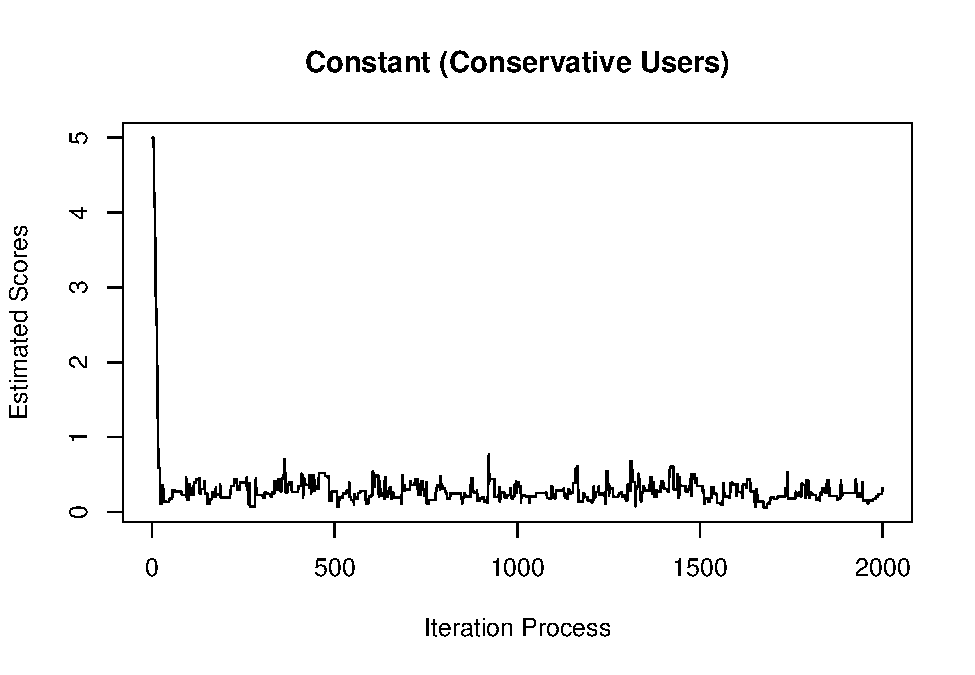
\includegraphics{bookdown-demo_files/figure-latex/unnamed-chunk-5-1.pdf}

\begin{Shaded}
\begin{Highlighting}[]
\KeywordTok{plot}\NormalTok{(fit_C}\OperatorTok{$}\NormalTok{theta[,}\DecValTok{2}\NormalTok{],}\DataTypeTok{main=}\StringTok{"Estimated Ideology Scores (Conservative Users)"}\NormalTok{,}
     \DataTypeTok{xlab=}\StringTok{"Iteration Process"}\NormalTok{,}\DataTypeTok{ylab=}\StringTok{"Ideology Scores"}\NormalTok{,}\DataTypeTok{type=}\StringTok{"l"}\NormalTok{)}
\end{Highlighting}
\end{Shaded}

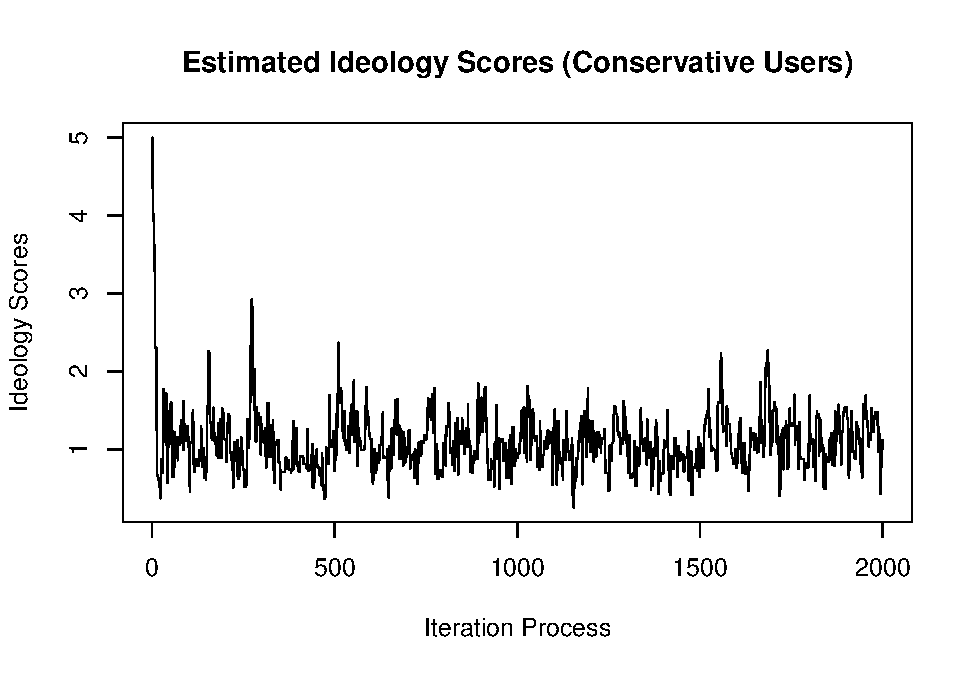
\includegraphics{bookdown-demo_files/figure-latex/unnamed-chunk-5-2.pdf}

\begin{Shaded}
\begin{Highlighting}[]
\KeywordTok{hist}\NormalTok{(fit_C}\OperatorTok{$}\NormalTok{theta[,}\DecValTok{2}\NormalTok{],}\DataTypeTok{main=}\StringTok{"Estimated Ideology Scores (Conservative Users)"}\NormalTok{,}
     \DataTypeTok{xlab=}\StringTok{"Ideology Scores"}\NormalTok{,}\DataTypeTok{breaks =} \DecValTok{100}\NormalTok{)}
\end{Highlighting}
\end{Shaded}

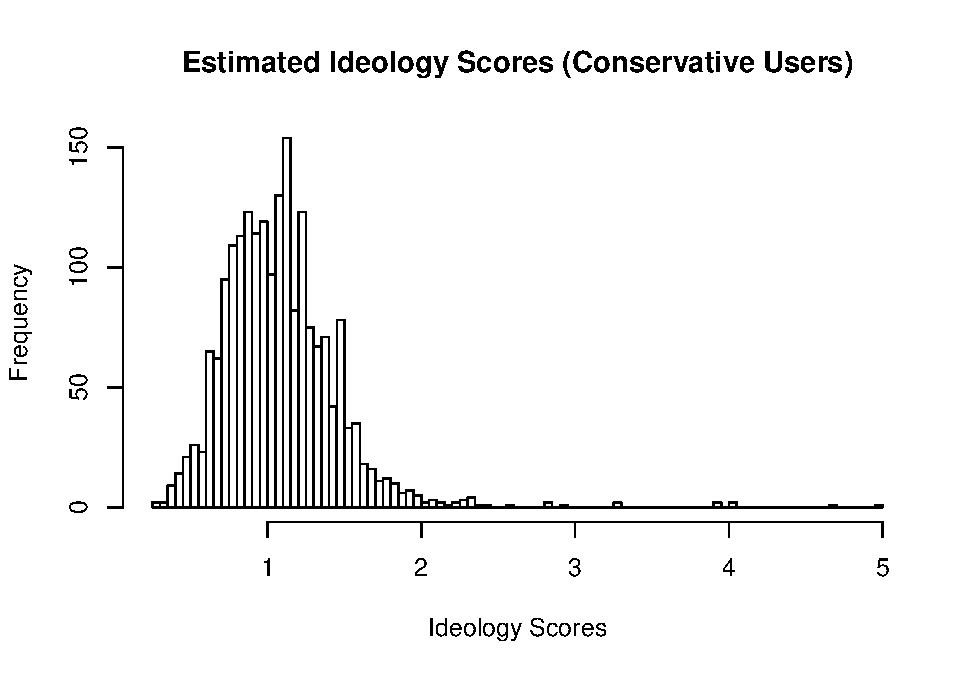
\includegraphics{bookdown-demo_files/figure-latex/unnamed-chunk-5-3.pdf}

\section{Simulating Data of Liberal Users on Twitter and Model
Testing}\label{simulating-data-of-liberal-users-on-twitter-and-model-testing}

To further verify the Metropolis Hastings algorithm, I plan to test the
opposite estimate. Specifically, assume that we observe another user,
who is more liberal. To simulate Twitter following data for this user, I
assign this user to follow more Democrat senators. In this case, we
would expect to see a negative value for their estimated ideology. As we
can see in the histogram shown below, as expected, the estimated value
is negative, providing convergent evidence for the model and the
algorithm.

\begin{Shaded}
\begin{Highlighting}[]
\CommentTok{#This user approximately follows 10 Republican Senators and 45 Democrat Senators. }
\NormalTok{Data_user<-}\KeywordTok{as.data.frame}\NormalTok{(}\KeywordTok{matrix}\NormalTok{(}\KeywordTok{c}\NormalTok{(}\KeywordTok{ifelse}\NormalTok{(}\KeywordTok{runif}\NormalTok{(}\DecValTok{50}\NormalTok{)}\OperatorTok{<}\NormalTok{.}\DecValTok{8}\NormalTok{,}\DecValTok{0}\NormalTok{,}\DecValTok{1}\NormalTok{),}\KeywordTok{ifelse}\NormalTok{(}\KeywordTok{runif}\NormalTok{(}\DecValTok{50}\NormalTok{)}\OperatorTok{<}\NormalTok{.}\DecValTok{1}\NormalTok{,}\DecValTok{0}\NormalTok{,}\DecValTok{1}\NormalTok{))), }\DecValTok{100}\NormalTok{, }\DecValTok{1}\NormalTok{)}
\KeywordTok{colnames}\NormalTok{(Data_user)<-}\KeywordTok{c}\NormalTok{(}\StringTok{"L_User"}\NormalTok{)}
\NormalTok{Data_combined<-}\KeywordTok{cbind}\NormalTok{(Data_Elites,Data_user)}

\NormalTok{X_data<-Data_combined}\OperatorTok{$}\NormalTok{Elite_ideology}
\NormalTok{Y_data<-Data_combined}\OperatorTok{$}\NormalTok{L_User}


\NormalTok{fit_L<-}\KeywordTok{Bayes_logit}\NormalTok{(Y_data,X_data)}
\NormalTok{fit_L}\OperatorTok{$}\NormalTok{acceptance_rate}
\end{Highlighting}
\end{Shaded}

\begin{verbatim}
## [1] 0.09904952 0.80140070
\end{verbatim}

\begin{Shaded}
\begin{Highlighting}[]
\KeywordTok{plot}\NormalTok{(fit_L}\OperatorTok{$}\NormalTok{theta[,}\DecValTok{1}\NormalTok{],}\DataTypeTok{main=}\StringTok{"Constant (Liberal Users)"}\NormalTok{,}
     \DataTypeTok{xlab=}\StringTok{"Iteration Process"}\NormalTok{,}\DataTypeTok{ylab=}\StringTok{"Estimated Scores"}\NormalTok{,}\DataTypeTok{type=}\StringTok{"l"}\NormalTok{)}
\end{Highlighting}
\end{Shaded}

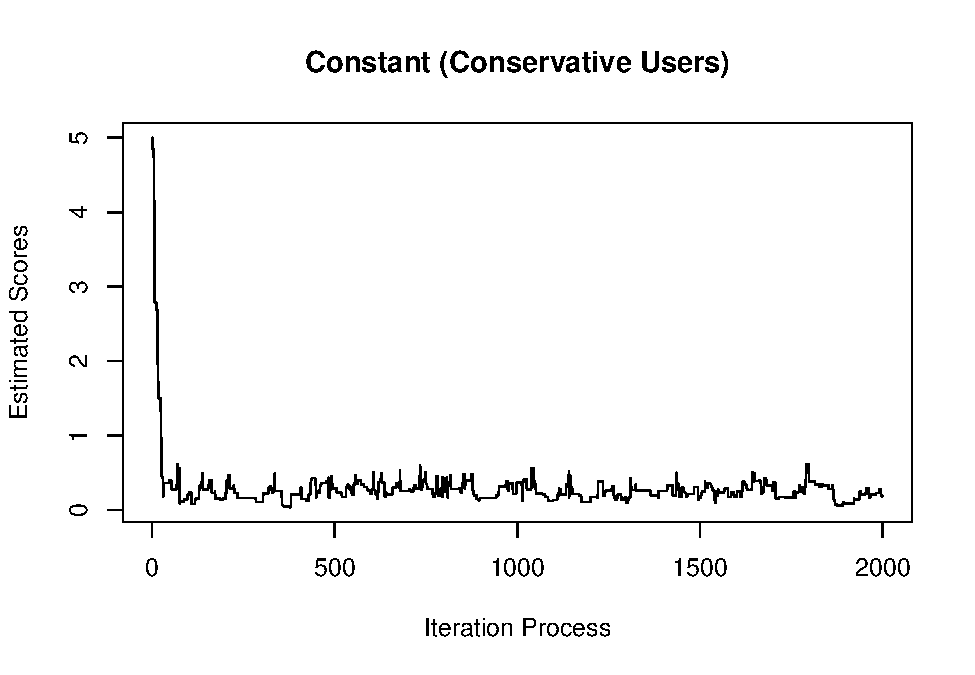
\includegraphics{bookdown-demo_files/figure-latex/unnamed-chunk-6-1.pdf}

\begin{Shaded}
\begin{Highlighting}[]
\KeywordTok{plot}\NormalTok{(fit_L}\OperatorTok{$}\NormalTok{theta[,}\DecValTok{2}\NormalTok{],}\DataTypeTok{main=}\StringTok{"Estimated Ideology Scores (Liberal Users)"}\NormalTok{,}
     \DataTypeTok{xlab=}\StringTok{"Iteration Process"}\NormalTok{,}\DataTypeTok{ylab=}\StringTok{"Ideology Scores"}\NormalTok{,}\DataTypeTok{type=}\StringTok{"l"}\NormalTok{)}
\end{Highlighting}
\end{Shaded}

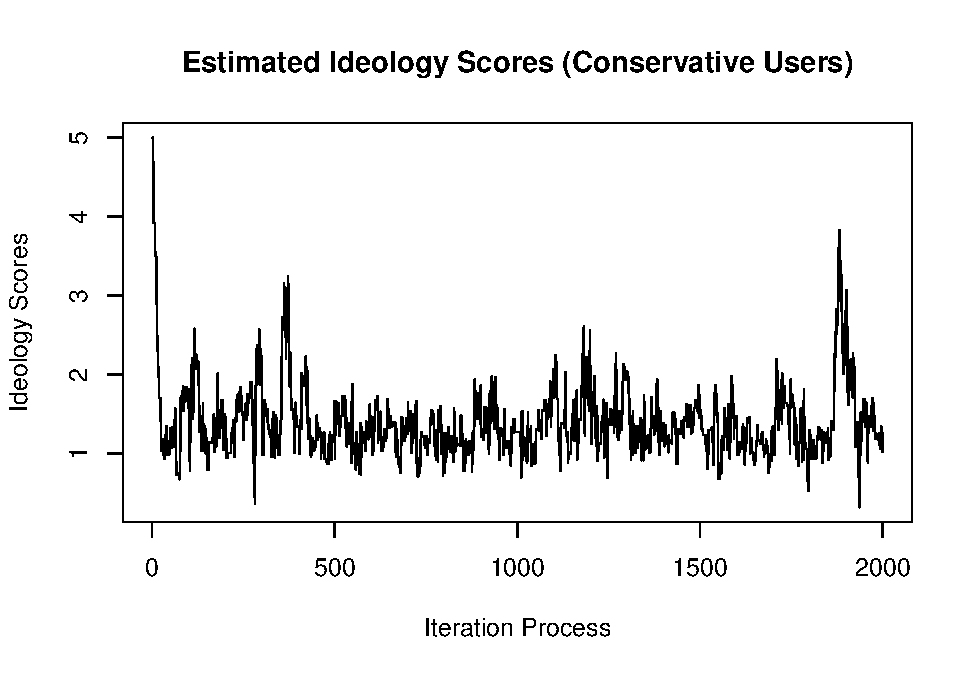
\includegraphics{bookdown-demo_files/figure-latex/unnamed-chunk-6-2.pdf}

\begin{Shaded}
\begin{Highlighting}[]
\KeywordTok{hist}\NormalTok{(fit_L}\OperatorTok{$}\NormalTok{theta[,}\DecValTok{2}\NormalTok{],}\DataTypeTok{main=}\StringTok{"Estimated Ideology Scores (Liberal Users)"}\NormalTok{,}
     \DataTypeTok{xlab=}\StringTok{"Ideology Scores"}\NormalTok{,}\DataTypeTok{breaks =} \DecValTok{100}\NormalTok{)}
\end{Highlighting}
\end{Shaded}

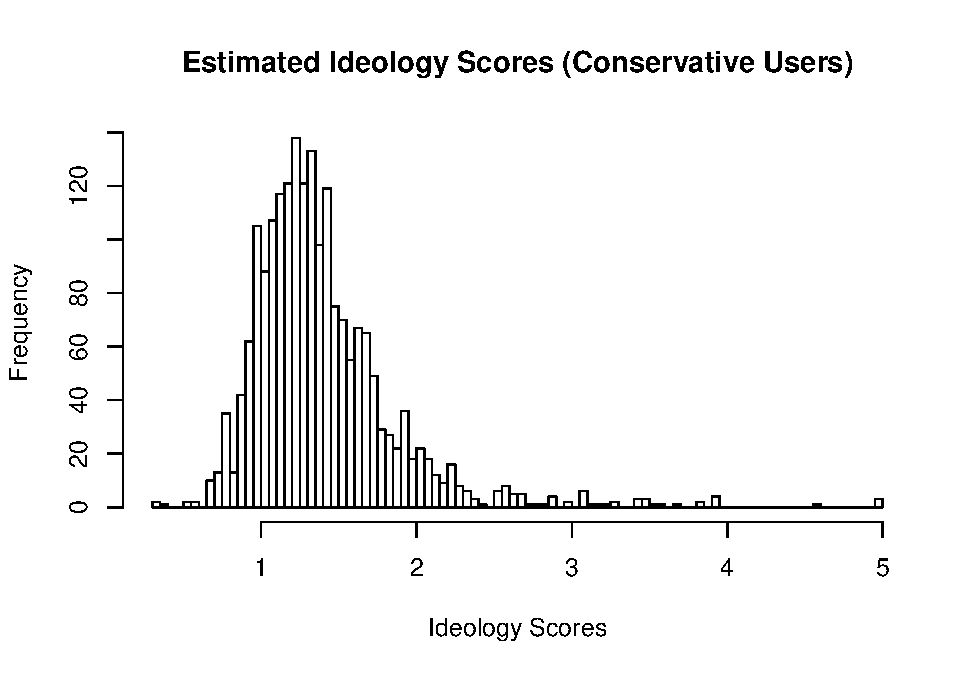
\includegraphics{bookdown-demo_files/figure-latex/unnamed-chunk-6-3.pdf}

\chapter{Linear Mixed Models}\label{linear-mixed-models}

The following code generates 4 numbers (\(N(0,10)\)) for 4 groups. Then,
replicate it within each group.That is, in the end, there are 8
observations.

Note that, in the following code, there are no ``independent
variables''. Both the linear model and mixed model are actually just
trying to calculate the mean.

\begin{Shaded}
\begin{Highlighting}[]
\CommentTok{# The original R code: http://www.john-ros.com/Rcourse/lme.html}
\CommentTok{# I did some minor changes and added some additional comments.}

\KeywordTok{set.seed}\NormalTok{(}\DecValTok{123}\NormalTok{)}
\NormalTok{n.groups <-}\StringTok{ }\DecValTok{4} \CommentTok{# number of groups}
\NormalTok{n.repeats <-}\StringTok{ }\DecValTok{2} \CommentTok{# samples per group}
\CommentTok{#Generating index for observations belong to the same group}
\NormalTok{groups <-}\StringTok{ }\KeywordTok{as.factor}\NormalTok{(}\KeywordTok{rep}\NormalTok{(}\DecValTok{1}\OperatorTok{:}\NormalTok{n.groups, }\DataTypeTok{each=}\NormalTok{n.repeats))}
\NormalTok{n <-}\StringTok{ }\KeywordTok{length}\NormalTok{(groups)}
\CommentTok{#Generating 4 random numbers, assuming normal distribution}
\NormalTok{z0 <-}\StringTok{ }\KeywordTok{rnorm}\NormalTok{(n.groups, }\DecValTok{0}\NormalTok{, }\DecValTok{10}\NormalTok{) }
\NormalTok{(z <-}\StringTok{ }\NormalTok{z0[}\KeywordTok{as.numeric}\NormalTok{(groups)]) }\CommentTok{# generate and inspect random group effects}
\end{Highlighting}
\end{Shaded}

\begin{verbatim}
## [1] -5.6047565 -5.6047565 -2.3017749 -2.3017749 15.5870831 15.5870831  0.7050839
## [8]  0.7050839
\end{verbatim}

\begin{Shaded}
\begin{Highlighting}[]
\NormalTok{epsilon <-}\StringTok{ }\KeywordTok{rnorm}\NormalTok{(n,}\DecValTok{0}\NormalTok{,}\DecValTok{1}\NormalTok{) }\CommentTok{# generate measurement error}
\NormalTok{beta0 <-}\StringTok{ }\DecValTok{2} \CommentTok{# this is the actual parameter of interest! The global mean.}
\NormalTok{y <-}\StringTok{ }\NormalTok{beta0 }\OperatorTok{+}\StringTok{ }\NormalTok{z }\OperatorTok{+}\StringTok{ }\NormalTok{epsilon }\CommentTok{# sample from an LMM}

\CommentTok{# fit a linear model assuming independence}
\CommentTok{# i.e., assume that there is no "group things".}
\NormalTok{lm.}\DecValTok{5}\NormalTok{ <-}\StringTok{ }\KeywordTok{lm}\NormalTok{(y}\OperatorTok{~}\DecValTok{1}\NormalTok{)}

\CommentTok{# fit a mixed-model that deals with the group dependence}
\CommentTok{#install.packages("lme4")}
\KeywordTok{library}\NormalTok{(lme4)}
\NormalTok{lme.}\DecValTok{5}\NormalTok{ <-}\StringTok{ }\KeywordTok{lmer}\NormalTok{(y}\OperatorTok{~}\DecValTok{1}\OperatorTok{|}\NormalTok{groups) }
\end{Highlighting}
\end{Shaded}

\chapter{Generalized Linear Mixed
Models}\label{generalized-linear-mixed-models}

The following is the note from Charle E. McCulloch's ``Maximum
likelihood algorithems for Generalized Linear Mixed Models''

\bibliography{book.bib,packages.bib}

\end{document}
